\subsubsection{Ballnachschub}
\begin{figure}[h!]
	\centering
	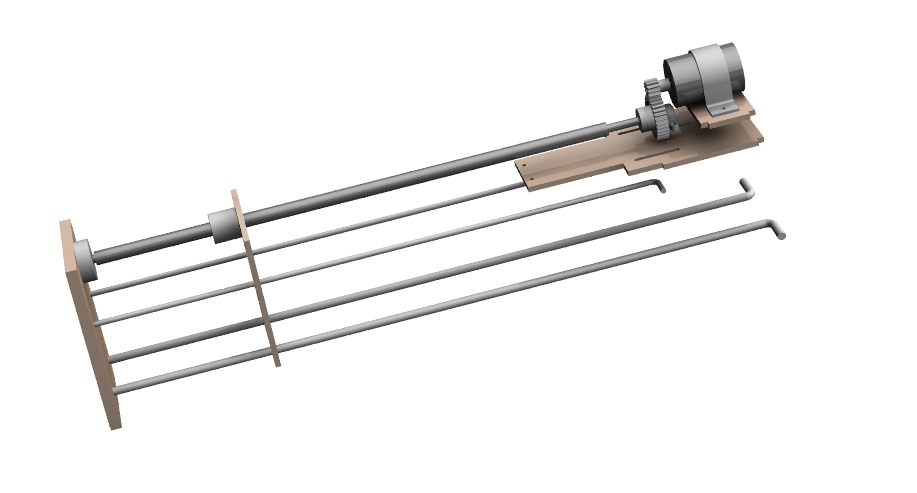
\includegraphics[width=\linewidth]{../../fig/Ballnachschub}
	\caption{Ballnachschub}
	\label{fig:Ballnachschub}
\end{figure}
\paragraph{Komponentenbeschrieb}

Der Ballnachschub wird mittels einer rotierenden Trapezgewindespindel (TR10x3) und einem Mitnehmer sichergestellt. Die Tennisbälle werden seitlich mit Alustangen geführt und so in Richtung der Abwurfvorrichtung transportiert. Die Trapezgewindespindel ist auf der Unterseite mit einem Rillenkugellager gelagert. Auf der Oberseite wird die Lagerung mit einem Stehlager aus Kunststoff der Firma Igus realisiert. Ein DC-Motor treibt die Trapezgewindespindel an. Die Kraftübertragung vom DC-Motor auf die Trapezgewindespindel erfolgt mit zwei Kunststoff Stirnrädern. Das Übersetzungsverhältnis hierbei beträgt 2.67. 

\paragraph{Entwicklungsprozess}

In einem ersten Entwurf wurde die Trapezgewindeführung auf der Unterseite auch mit einer Gleitführung realisiert. Dies funktionierte für den Ballnachschub einwandfrei. Wurde nach dem Ballabwurf die Drehrichtung umgekehrt, um den Mitnehmer wieder in die Startposition zu bringen ergaben sich einige Probleme. Wegen der realisierten Gleitführung, konnte sich die Trapezgewindespindel in axialer Richtung frei bewegen. Dies führte dazu, dass die Spindel beim Zurückstellen tendenziell nach oben gezogen wurde. Dies führte zu Schwingungen, welche ein automatisches Zurückfahren verunmöglichte. Mit der angepassten Lagerung war dieses Problem behoben. 
Eine weitere Knacknuss war die Führung der Bälle und dadurch das Finden der optimalen Position für die Führungsstangen. Da Tennisbälle eine runde Form besitzen, neigen sie dazu sich gegenseitig wegzudrücken. Dadurch mussten wir den Durchmesser der Aluminiumführungsstangen vergrössern. Beim ersten Entwurf endeten alle Führungsstangen auf der Höhe des Drehrades. Dies führte dazu dass die Tennisbälle nach dem Abwurf unsere Maschine auf einer horizontalen Flugbahn verliessen und nicht wie vorgesehen unter einem Winkel von 45° zur Horizontalen. Dieses Problem konnte durch einer Verlängerung der Führungsstangen bis nach dem Drehrad verhindert werden. 
Der DC Motor wurde mit einer Rohrschelle befestigt. Dabei wurde die Platte, auf welcher die Rohrschelle befestigt ist, im richtigen Abstand positioniert, so dass die Übersetzung realisiert werden kann. Dies stellt keine optimale Lösung dar. Da die Funktion aber gegeben war, wurde auf eine Verbesserung verzichtet. 
